%----------------------------------------------------------
\usepackage{amsfonts}
\usepackage{amsmath}
\usepackage{MnSymbol}
%----------------------------------------------------------
%\newcommand{\doclicense}{\copyright\xspace}
%\newcommand{\doclicense}{\ccLogo\ccAttribution\xspace}%\ccShareAlike
\newcommand{\doclicense}{\includegraphics[width=0.1\textwidth]{doc-spec/by.eps}\xspace}%\ccShareAlike
%----------------------------------------------------------
\usepackage[T2A]{fontenc}
\usepackage[utf8]{inputenc}
\usepackage[english,russian]{babel} %% это необходимо для включения переносов
\usepackage{float}
\usepackage{algpseudocode}      % для окружения algorithmic
\usepackage{algorithm}          % для нумерации алгоритмов

\usepackage{listings}
\usepackage{longtable}
\usepackage{rotating}
\usepackage{multirow}
\usepackage{pdflscape}
\usepackage{bm}
\usepackage{cmap} % необходимо для возможности копирования и поиска в готовом PDF
\usepackage{array}
\usepackage{multicol}

\usepackage[normalem]{ulem}

%-------------------------
% определение атрибутов сборки Git
\usepackage[grumpy, maxdepth=6]{gitinfo2}
\renewcommand{\gitMark}{[git] \textbullet{} \gitBranch\,@\,\gitAbbrevHash{} \textbullet{} \gitAuthorName, \gitAuthorEmail (\gitAuthorIsoDate)}
%-------------------------
\newcommand{\authorSID}{\Year, \AllAuthors, \pdftexbanner, \jobname}
%-------------------------
\newcommand{\authorSIDfooter}[1][white]{\begin{tabular}{c}\thepage\\[-6pt]\textcolor{#1}{\tiny\authorSID}\\[-6pt]\textcolor{#1}{\tiny\gitMark}\end{tabular}}
%-------------------------
%\newcommand{\authorSIDright}{\begin{tabular}{c}\tiny\authorSID\\\tiny\gitMark\end{tabular}}
\newcommand{\authorSIDright}{\textcolor{gray!10.0}{\tiny\gitMark}}
%-------------------------
% Сохранение метаданных в PDF об авторе документа
\usepackage{hyperxmp}
\usepackage{hyperref}
\hypersetup{%
%    bookmarks=false,        % show bookmarks bar?
    pdftoolbar=true,        % show Acrobat’s toolbar?
    pdfmenubar=true,        % show Acrobat’s menu?
    pdffitwindow=false,     % window fit to page when opened
    pdfstartview={FitH},    % fits the width of the page to the window
    pdftitle={\Title},    	% title
    pdfauthor={\AllAuthors},    % author
%		pdfcopyright={Copyright © \Year, \Author. Все права защищены.},
		pdfcopyright={CC BY 4.0, \Year, \AllAuthors.},
		pdflicenseurl={http://creativecommons.org/licenses/by/4.0/},
    pdfsubject={\SubjectOfResearch},   % subject of the document
    pdfcreator={\pdftexbanner},   % creator of the document
%		pdfpublisher={Computer-aided design department, Bauman Moscow State Technical University},
		pdfcaptionwriter={Ass. Prof., PhD. Alexandr P. Sokolov},
    pdfproducer={\AllAuthors(\gitAuthorEmail), \Year, Computer-aided design department, Bauman Moscow State Technical University}, % producer of the document
    pdfkeywords={\keywordsru, \keywordsen}, % ключевые слова
    pdfnewwindow=true,      % links in new window
    colorlinks=true,
    citecolor=purple,
    linkcolor=red,      % color of internal links (change box color with linkbordercolor)
    urlcolor=green,
    filecolor=black      % color of file links
}
%----------------------------------------------------------
\usepackage[style=long4colheader, translate=babel, section=section]{glossaries}
\usepackage[abbreviations, toc=true, xindy, automake]{glossaries-extra}
\setglossarystyle{treenoname}%+
\makeglossaries
%----------------------------------------------------------
% добавление поддержки команды вывода текста на полях \marginnote
\usepackage{marginnote}
% добавление поддержки команды \color
\usepackage{xcolor}
%--------------------------------------------
% final - удаляет все всплывающие комментарии
\usepackage[author={Alexandr Sokolov},opacity=0.1]{pdfcomment}
%\usepackage[author={Alexandr Sokolov},opacity=0.1,final]{pdfcomment}
\newcommand{\messnote}[1]{\marginnote{\color[rgb]{1,0,0}\Huge\textbf{!}\pdfcomment{#1}}[-1.0cm]}

\usepackage{pdfpages}
%----------------------------------------------------------------
\includepdfset{turn=true,scale=0.9,pages=-,pagecommand={\pagestyle{fancy}}}
%----------------------------------------------------------
% необходимо для работы команды \xspace (умный пробел после замены, осуществляемой некоторой командой в тексте)
\usepackage{xspace}

\usepackage{tikz}
\usetikzlibrary{tikzmark}
%\usetikzlibrary{matrix,automata,graphs}
\usetikzlibrary{arrows,positioning,trees}

%----------------------------------------------------------
% необходимо для возможности включать в имена включаемых файлов _
\usepackage[strings]{underscore}
%----------------------------------------------------------
% Произвольная нумерация списков.
\usepackage{enumerate}
%----------------------------------------------------------
\raggedbottom
\textwidth=163mm
\textheight=220mm
\oddsidemargin=-0.5pt
\footskip=30pt
\headheight=28pt
\headsep=25pt
\topskip=10pt
\baselineskip=15pt
\topmargin=-4mm
%----------------------------------------------------------
\def\notedate{\date}
% Настройки колонтитулов
\usepackage{fancyhdr} % Headers and footers
\pagestyle{fancy} % All pages have headers and footers
\fancyhf{} % clear all headers and footers - equivalent to %\fancyhead{} and \fancyfoot{}
\renewcommand{\headrulewidth}{0.2pt}
\renewcommand{\footrulewidth}{0.2pt}
\newcommand{\mymarks}{%
    \ifthenelse{\equal{\rightmark}{}} % is \rightmark empty?
        {\leftmark} % when empty
        {\itshape\notedate: \rightmark~(\currentauthor)} % when not empty
}
\renewcommand{\sectionmark}[1]{\markboth{\thesection.\ #1}{}}
\renewcommand{\subsectionmark}[1]{\markright{#1}}

\fancyhead[C]{\mymarks}
\fancyfoot[C]{\authorSIDfooter[white]}
%\fancyfoot[C]{\thepage}
%----------------------------------------------------------
\usepackage[hpos=0.98\paperwidth, % .98 to prevent bleed
            vpos=0.7\paperwidth,
            angle=90]{draftwatermark}

\SetWatermarkText{\authorSIDright}
%\SetWatermarkColor[gray]{0.1}
\SetWatermarkFontSize{0.2cm}
\SetWatermarkAngle{90}
\SetWatermarkHorCenter{20cm}
%----------------------------------------------------------
% указание
\setcounter{secnumdepth}{2}
%----------------------------------------------------------
% подлкючение пакета для подсчета объектов
\usepackage{totcount}
% регистрируем счетчик страниц
\regtotcounter{page}
%----------------------------------------------------------
% необходимо для того, чтобы в окружениях enumerate можно было менять формат нумерации
% необходимо для работы опции wide в окружениях enumerate
\usepackage{enumitem}
%\setlist{noitemsep, nosep, wide}% topsep=0pt, bottomsep=0pt}
\setenumerate{noitemsep, nosep, wide}% topsep=0pt, bottomsep=0pt}
\renewcommand\labelitemi{--}

%----------------------------------------------------------
%Необходимо для сокращения размера шрифта подписей и сокращения отступов между рисунком и подписью к нему
\usepackage[margin=5pt,font={small, singlespacing}, labelfont={small}, justification=centering, labelsep=period]{caption}
\captionsetup{belowskip=0pt}
%----------------------------------------------------------
\usepackage[numbers]{natbib}
\usepackage{bibentry}
%***natbib, bibentry***%
% Следующий код необходим для того, чтобы исправить конфликт между пакетами natbib+bibentry и стилем оформления ссылок согласно российскому ГОСТу cp1251gost705u
\ifx\undefined\selectlanguageifdefined
\def\selectlanguageifdefined#1{}\else\fi
\ifx\undefined\BibEmph
\def\BibEmph#1{\emph{#1}}\else\fi
%--------------------------------------------
\usepackage{tikz}
\usetikzlibrary{tikzmark}
\usetikzlibrary{trees, calc, automata}
\usetikzlibrary{arrows,arrows.meta, shapes}
\usetikzlibrary{positioning}
%--------------------------------------------
% подключение листингов и определение языков
\usepackage{listings}

\lstset
{
		extendedchars=\true, % включаем не латиницу
%		inputencoding=utf8x,
		frame=tb, % рамка сверху и снизу
		escapechar=|, % |«выпадаем» в LATEX|
		xleftmargin=0.5cm,
		xrightmargin=0.5cm,
		columns=fullflexible,
%		aboveskip=5pt,
		numbers=left,                    % where to put the line-numbers; possible values are (none, left, right)
		numbersep=4pt,                   % how far the line-numbers are from the code
		showspaces=false,
		showstringspaces=false,
		breakatwhitespace=true,         % sets if automatic breaks should only happen at whitespace
		breaklines=true,                 % sets automatic line breaking
		basicstyle=\color{black}\small\sffamily,%\ttfamily,% \sffamily
		commentstyle=\color{gray}\itshape, % шрифт для комментариев
		stringstyle=\color{orange},
%		stringstyle=\bfseries, % шрифт для строк
		numberstyle=\footnotesize\color{gray},
%		numberstyle=\ttfamily\small\color{gray}, % the style that is used for the line-numbers
		keywordstyle=\color{blue}\bfseries,
%		directivestyle=\color{red},
%		emph={int,char,double,float,unsigned,bool,string},
		emphstyle={\color{blue}\bfseries},
		tabsize=2,
%		morecomment=[l]{//},
%		otherkeywords={=,==,:,&},
		texcl=true,
}

%----------------------------------------------------------
% Подписи к листингам на русском языке.
\renewcommand\lstlistlistingname{\cyr\CYRL\cyri\cyrs\cyrt\cyri\cyrn\cyrg\cyri}

\lstloadlanguages{Python, [LaTeX]TeX, bash, XML, make, C++}

\usepackage{xcolor}

\colorlet{punct}{red!60!black}
\definecolor{background}{HTML}{EEEEEE}
\definecolor{delim}{RGB}{20,105,176}
\colorlet{numb}{magenta!60!black}

\lstdefinelanguage{json}{%
    basicstyle=\normalfont\ttfamily,
    numbers=left,
    numberstyle=\scriptsize,
    stepnumber=1,
    numbersep=8pt,
    showstringspaces=false,
    breaklines=true,
    frame=lines,
    backgroundcolor=\color{background},
    literate=
     *{0}{{{\color{numb}0}}}{1}
      {1}{{{\color{numb}1}}}{1}
      {2}{{{\color{numb}2}}}{1}
      {3}{{{\color{numb}3}}}{1}
      {4}{{{\color{numb}4}}}{1}
      {5}{{{\color{numb}5}}}{1}
      {6}{{{\color{numb}6}}}{1}
      {7}{{{\color{numb}7}}}{1}
      {8}{{{\color{numb}8}}}{1}
      {9}{{{\color{numb}9}}}{1}
      {:}{{{\color{punct}{:}}}}{1}
      {,}{{{\color{punct}{,}}}}{1}
      {\{}{{{\color{delim}{\{}}}}{1}
      {\}}{{{\color{delim}{\}}}}}{1}
      {[}{{{\color{delim}{[}}}}{1}
      {]}{{{\color{delim}{]}}}}{1},
}

\lstdefinelanguage{TmlSyntax}
{
		extendedchars=\true,
%		texcl=\true,
    basicstyle=\sffamily\scriptsize,
		frame=single,
		numbers=left, % where to put the line-numbers; possible values are (none, left, right)
    numbersep=4pt, % how far the line-numbers are from the code
		xleftmargin=0.5cm,
		xrightmargin=0.5cm,
		breakatwhitespace=true,         % sets if automatic breaks should only happen at whitespace
    numberstyle=\small\color{gray}, % the style that is used for the line-numbers
    columns=fullflexible,
    morecomment=[s][\color{blue}\bfseries]{@}{@},
    morecomment=[l]{-},
    otherkeywords={=,|,(,)},
    keywordstyle={\color{brown}\bfseries},
    commentstyle=\color{gray}\itshape
}

\lstdefinelanguage{BNFSyntax}%
{%
		extendedchars=\true,
%		texcl=true,
		escapechar=>, % |«выпадаем» в LATEX|
		frame=tb, % рамка сверху и снизу
    columns=fullflexible,
		numbers=left, % where to put the line-numbers; possible values are (none, left, right)
    numbersep=4pt, % how far the line-numbers are from the code
		xleftmargin=0.5cm,
		xrightmargin=0.5cm,
		showspaces=\false,
		showstringspaces=\false,
		breakatwhitespace=true,         % sets if automatic breaks should only happen at whitespace
		breaklines=true,                 % sets automatic line breaking
		basicstyle=\color{black}\small\sffamily,
    numberstyle=\footnotesize\color{gray}, % the style that is used for the line-numbers
    keywordstyle={\color{black}\bfseries},
		commentstyle=\color{gray}\itshape, % шрифт для комментариев
		stringstyle=\color{orange}, % шрифт для строк
    morecomment=[s][\color{blue}]{'}{'},
		keywords={ID,TEXT,NUM},%, edge_id, binname, entry_func, strategy, parallelization, branching},
    morecomment=[l]{//},
		tabsize=2,
		literate=
		{=}{\textcolor{blue}{=}\bfseries}1%
}

\lstdefinelanguage{nginx}%
{%
		extendedchars=\true,
		escapechar=>, % |«выпадаем» в LATEX|
		frame=tb, % рамка сверху и снизу
    columns=fullflexible,
		numbers=left, % where to put the line-numbers; possible values are (none, left, right)
    numbersep=4pt, % how far the line-numbers are from the code
		xleftmargin=0.5cm,
		xrightmargin=0.5cm,
		showspaces=\false,
		showstringspaces=\false,
		breakatwhitespace=true,         % sets if automatic breaks should only happen at whitespace
		breaklines=true,                 % sets automatic line breaking
		basicstyle=\color{black}\small\sffamily,
    numberstyle=\footnotesize\color{gray}, % the style that is used for the line-numbers
    keywordstyle={\color{black}\bfseries},
		commentstyle=\color{gray}\itshape, % шрифт для комментариев
		stringstyle=\color{orange}, % шрифт для строк
    morecomment=[s][\color{blue}]{'}{'},
		keywords={upstream,server,listen,location},%, edge_id, binname, entry_func, strategy, parallelization, branching},
    morecomment=[l]{//},
		tabsize=2,
    literate=
     *{0}{{{\color{numb}0}}}{1}
      {1}{{{\color{numb}1}}}{1}
      {2}{{{\color{numb}2}}}{1}
      {3}{{{\color{numb}3}}}{1}
      {4}{{{\color{numb}4}}}{1}
      {5}{{{\color{numb}5}}}{1}
      {6}{{{\color{numb}6}}}{1}
      {7}{{{\color{numb}7}}}{1}
      {8}{{{\color{numb}8}}}{1}
      {9}{{{\color{numb}9}}}{1}
      {;}{{{\color{punct}{;}}}}{1}
      {:}{{{\color{punct}{:}}}}{1}
      {\$}{{{\color{punct}{\$}}}}{1}
      {/}{{{\color{punct}{/}}}}{1}
      {\{}{{{\color{delim}{\{}}}}{1}
      {\}}{{{\color{delim}{\}}}}}{1},
}

\lstdefinelanguage{aINIExample}%
{%
		extendedchars=\true,
    basicstyle=\sffamily\small,
%		texcl=\true, % необходимо для того, чтобы пакет listings не ругался при компиляции UTF8 материала при содержании кирилических символов в комментариях
		escapechar=\#, % |«выпадаем» в LATEX|
		frame=tb, % рамка сверху и снизу
    columns=fullflexible,
		numbers=left, % where to put the line-numbers; possible values are (none, left, right)
    numbersep=5pt,% how far the line-numbers are from the code
    numberstyle=\small\color{gray}, % the style that is used for the line-numbers
		breakatwhitespace=true,         % sets if automatic breaks should only happen at whitespace
    morecomment=[s][\color{black}\bfseries]{[}{]},
    morecomment=[s][\color{purple}\bfseries]{=[}{]},
    morecomment=[s][\color{pink}\bfseries]{[[}{]]},
    morecomment=[s][\color{blue}\bfseries]{@}{@},
    morecomment=[l]{//},
    commentstyle=\color{gray}\itshape,
    otherkeywords={=,\$,-,*},
    keywordstyle={\color{brown}\bfseries}
%		literate=
%		{[}{\textcolor{brown}{[}}1
%		{]}{\textcolor{brown}{]}}1
%		{*}{\textcolor{brown}\bfseries{*}}1
}

\lstdefinelanguage{aDOTExample}%
{
		extendedchars=\true,
		escapechar=\#,
%		texcl=\true, этот параметр криво работает - удаляет все пробелы из комментариев
    basicstyle=\sffamily\small,
		frame=tb, % рамка сверху и снизу
    columns=fullflexible,
		numbers=left, % where to put the line-numbers; possible values are (none, left, right)
    numbersep=4pt, % how far the line-numbers are from the code
		xleftmargin=0.5cm,
		xrightmargin=0.5cm,
    numberstyle=\small\color{gray}, % the style that is used for the line-numbers
		breakatwhitespace=true,         % sets if automatic breaks should only happen at whitespace
		showstringspaces=false,
		showspaces=false,
		morestring=[b]{"},
		stringstyle=\color{orange}, % шрифт для строк
		morecomment=[s][\color{gray}\bfseries]{[}{]},
    morecomment=[s][\color{blue}\bfseries]{__}{__},
    morecomment=[l]{//},
		keywords={digraph, module, entry_func, keys_mapping, edge, predicate, function, morphism, morphisms, selector, parallelism, threading, pseudo-parallelism},
    keywordstyle={\color{black}\bfseries},
    commentstyle=\color{gray}\itshape,
    otherkeywords={},
		literate=
%		{\$}{\textcolor{brown}{\$}}1
		{=}{\textcolor{brown}{=}}1
		{->}{\textcolor{brown}{->}}1
		{=>}{\textcolor{brown}{=>}}1
		{[}{\textcolor{red}{[}}1
		{]}{\textcolor{red}{]}}1
}

\lstdefinelanguage{docker}{
  keywords={FROM, RUN, COPY, ADD, ENTRYPOINT, CMD,  ENV, ARG, WORKDIR, EXPOSE, LABEL, USER, VOLUME, STOPSIGNAL, ONBUILD, MAINTAINER},
  keywordstyle=\color{blue}\bfseries,
  identifierstyle=\color{black},
  sensitive=false,
  comment=[l]{\#},
  commentstyle=\color{purple}\ttfamily,
  stringstyle=\color{red}\ttfamily,
  morestring=[b]',
  morestring=[b]"
}

\lstdefinelanguage{docker-compose}{
  keywords={image, environment, ports, container_name, ports, volumes, links},
  keywordstyle=\color{blue}\bfseries,
  identifierstyle=\color{black},
  sensitive=false,
  comment=[l]{\#},
  commentstyle=\color{purple}\ttfamily,
  stringstyle=\color{red}\ttfamily,
  morestring=[b]',
  morestring=[b]"
}
\lstdefinelanguage{docker-compose-2}{
  keywords={version, volumes, services},
  keywordstyle=\color{blue}\bfseries,
  keywords=[2]{image, environment, ports, container_name, ports, links, build},
  keywordstyle=[2]\color{olive}\bfseries,
  identifierstyle=\color{black},
  sensitive=false,
  comment=[l]{\#},
  commentstyle=\color{purple}\ttfamily,
  stringstyle=\color{red}\ttfamily,
  morestring=[b]',
  morestring=[b]"
}

%--------------------------------------------
% необходимо для команды \cancelto{0}{x}
\usepackage{cancel}
%----------------------------------------------------------
% необходимо для того, чтобы доопределить спецификатор P, для
% использования в таблицах при форматировании
\usepackage{array}
\newcolumntype{P}[1]{>{\centering\arraybackslash}p{#1}}
%----------------------------------------%
% необходимо для того, чтобы допускались разрывы страниц внутри align align*
\allowdisplaybreaks
%----------------------------------------%
%\def\pbs{\raggedright\baselineskip3.0ex}
\def\signhrule{\raggedright\baselineskip30.0ex \vrule height 0.5pt width30mm depth0pt}

\makeatletter
\def\dynscriptsize{\check@mathfonts\fontsize{\sf@size}{\z@}\selectfont}
\makeatother
\def\textunderset#1#2{\leavevmode
  \vtop{\offinterlineskip\halign{%
    \hfil##\hfil\cr\strut#2\cr\noalign{\kern-.3ex}
    \hidewidth\dynscriptsize\strut#1\hidewidth\cr}}}

\newcommand\executer[1]{\textunderset{\scriptsize{подпись, дата}}{\signvrule} #1}
%----------------------------------------------------------
% необходимо для поддержки поворотов текста
\usepackage[absolute]{textpos}
\setlength{\TPHorizModule}{30mm}
\setlength{\TPVertModule}{\TPHorizModule}
\textblockorigin{0mm}{25mm} % start everything near the top-left corner
%----------------------------------------%
% Определение отступа от номера в подсекции
\usepackage{tocloft}
\renewcommand\cftsubsecnumwidth{2.5cm}
%----------------------------------------------------------
% Определение заголовка заметки
%----------------------------------------------------------
% Пакеты для подсчета количества: страниц, и т.д.
\usepackage{etoolbox}
\usepackage{totcount,assoccnt}
%----------------------------------------------------------
% суперсчетчики всего ! :-)
\newtotcounter{csubsection}
\setcounter{csubsection}{0}
\def\oldsubsection{} \let\oldsubsection=\subsection
\def\subsection{\stepcounter{csubsection}\oldsubsection}

%\csname #1\endcsname\xspace

% Включение LaTeX заметки осуществляться в рамках подраздела уровня subsection
\newcommand{\notestatement}[2]{%
\subsection*{\notedate: #2}\expandafter\label{#1\arabic{csubsection}}
\addcontentsline{toc}{subsection}{\notedate:\hspace{10pt} #2}
}
% Включение PDF-заметки осуществляться НЕ в рамках подраздела уровня subsection,
% но с искусственным добавлением соответствующего залоговка в содержание
\newcommand{\pdfnotestatement}[2]{%
\markright{#2}\stepcounter{csubsection}\expandafter\label{#1\arabic{csubsection}}
\addcontentsline{toc}{subsection}{\notedate:\hspace{10pt} #2}%\rightmark}
}
%----------------------------------------------------------
% оформление "теорем"
%----------------------------------------------------------
\usepackage{amsthm}
\usepackage{thmtools}
%----------------------------------------------------------
\declaretheoremstyle[
  headfont=\normalfont\bfseries,
  numberwithin=section,
  bodyfont=\normalfont,%\itshape,
  spaceabove=1em plus 0.75em minus 0.25em,
  spacebelow=1em plus 0.75em minus 0.25em,
  headpunct={\newline},
  qed={$\sharp$},%\natural
]{theoremstyle}

\declaretheoremstyle[
  headfont=\normalfont\bfseries,
	numberwithin=section,
  bodyfont=\normalfont,
  spaceabove=1em plus 0.75em minus 0.25em,
  spacebelow=1em plus 0.75em minus 0.25em,
	headpunct={\newline},
  qed={$\natural$},%\sharp
]{vipremarkstyle}

\declaretheorem[
  style=vipremarkstyle,
  title=Важное замечание,
  refname={важное замечание,важные замечания},
  Refname={Важное замечание,Важные замечания}
]{vipremark}

%----------------------------------------------------------
\theoremstyle{theoremstyle}
%----------------------------------------------------------
\newtheorem{question}{Вопрос}
\newtheorem{task}{Задача}
\newtheorem{solution}{Решение}
\newtheorem{remark}{Замечание}
\newtheorem{theorem}{Теорема}
%--------------------------------------------------
\def\notedate{}
\def\currentauthor{}
%--------------------------------------------------
% атрибуты задачи
\newcommand{\noteattributes}[1]{%
\def\tempempty{}
\def\tempa{#1}
  \ifx\tempempty\tempa \def\tempa{\currentauthor, \notedate}\fi

\vspace{0.5cm}
\begin{flushright}
		\begin{tabular}{p{0.2\textwidth}p{0.45\textwidth}}
		\hfill Подготовлено: & \textit{\tempa} \\ %\doclicense~
		\end{tabular}
\end{flushright}
}
%----------------------------------------------------------
\DeclareMathOperator*{\argmax}{\arg\!\max}
%----------------------------------------------------------
\newcommand{\bs}[1]{\boldsymbol{#1}}
% #1 - current \doctype
% #2 - destination document
% #3 - text
\newcommand{\myconditionaltext}[3]%
{%
	\ifthenelse{\equal{#1}{avtoreferat}\AND\equal{#2}{avtoreferat}}{#3}{}% short version
	\ifthenelse{\equal{#1}{avtoreferat}\AND\equal{#2}{thesis}}{}{}% short version
	\ifthenelse{\equal{#1}{avtoreferat}\AND\equal{#2}{presentation}}{}{}% short version
	\ifthenelse{\equal{#1}{thesis}\AND\equal{#2}{presentation}}{}{}% short version
	\ifthenelse{\equal{#1}{thesis}\AND\equal{#2}{thesis}}{#3}{}% short version
	\ifthenelse{\equal{#1}{presentation}\AND\equal{#2}{presentation}}{#3}{}% short version
	\ifthenelse{\equal{#1}{presentation}\AND\equal{#2}{thesis}}{\pdfcomment{#3}}{}% short version
}
%----------------------------------------------------------
\newcommand{\mycitation}[2]{%
\noindent\colorbox{black!5}{\parbox{1.0\textwidth}{{\large\textbf{``}}\textit{#1}}}\linebreak
%\vspace{-5pt}
\parbox{1.0\textwidth}{\begin{flushright}#2\end{flushright}}
}
%----------------------------------------------------------
% указание на глубину вложенности подразделов при формировании содержания
\setcounter{secnumdepth}{2}
%----------------------------------------------------------
